\chapter{По мотивам CIM}

В данном разделе вводится описание конфигурации множества контролируемых параметров,
представленное с помощью конфигурационного файла и использованием расширяемого языка разметки XML, правил его оформления XSD.
Также приводится описание необходимых сущностей для представления
на программном уровне объектов предметной области.


\section{Определение Modbus тегов} \label{sec:modbus_tag}
Пример конфигурационного файла приведен в листинге \ref{lst:modbus_tags_example} в приложении \ref{app:sec:modbus_tag}.
Не смотря на то что в самом протоколе Modbus передаются только целые числа, некоторые производители Modbus-устройств,
в том числе производители средств разработки для программируемых логических контроллеров, расширяют возможности протокола
для передачи вещественных чисел одинарной и двойной точности, так и целочисленных значений размером до восьми байт \cite{book:gost:modbus_program_language}.

Каждый тег описывается тремя обязательными и двумя необязательными аттрибутами.
К обязательным относятся:
\begin{itemize}
    \item[\texttt{title}] заголовок тега, относящийся к предметной области;
    \item[\texttt{address}] адрес тега, согласованный с адресным пространством контроллера;
    \item[\texttt{type}] тип передаваемого значения, который может принимать следующие значения, в зависимости от группы:
    %
    \begin{itemize}
        \item[BOOL] 1 бит;
        \item[WORD] 16 бит;
        \item[DOUBLEWORD] 64 бита;
        \item[REAL] 32 бита;
        \item[LONGREAL] 64 бита.
    \end{itemize}
\end{itemize}
Необязательные аттрибуты служат для вспомогательной цели:
\begin{itemize}
    \item[\texttt{position}] первично -- определяет положение сигнального проводника на модуле в сборке контроллера;
    вторично -- обозначает, что это результат промежуточных вычислений контроллера;
    \item[\texttt{description}] описание передаваемого параметра.
\end{itemize}



\section{Иерархия классов}
На основе анализа предметной области строится иерархия классов для управления информационной моделью,
диаграмма взаимосвязи классов представлена на рисунке \ref{fig:modbus_class_uml} \cite[стр. 223]{book:oop:oop_analize}. 
\begin{landscape}
    \begin{center}
        \begin{figure}[h!]
            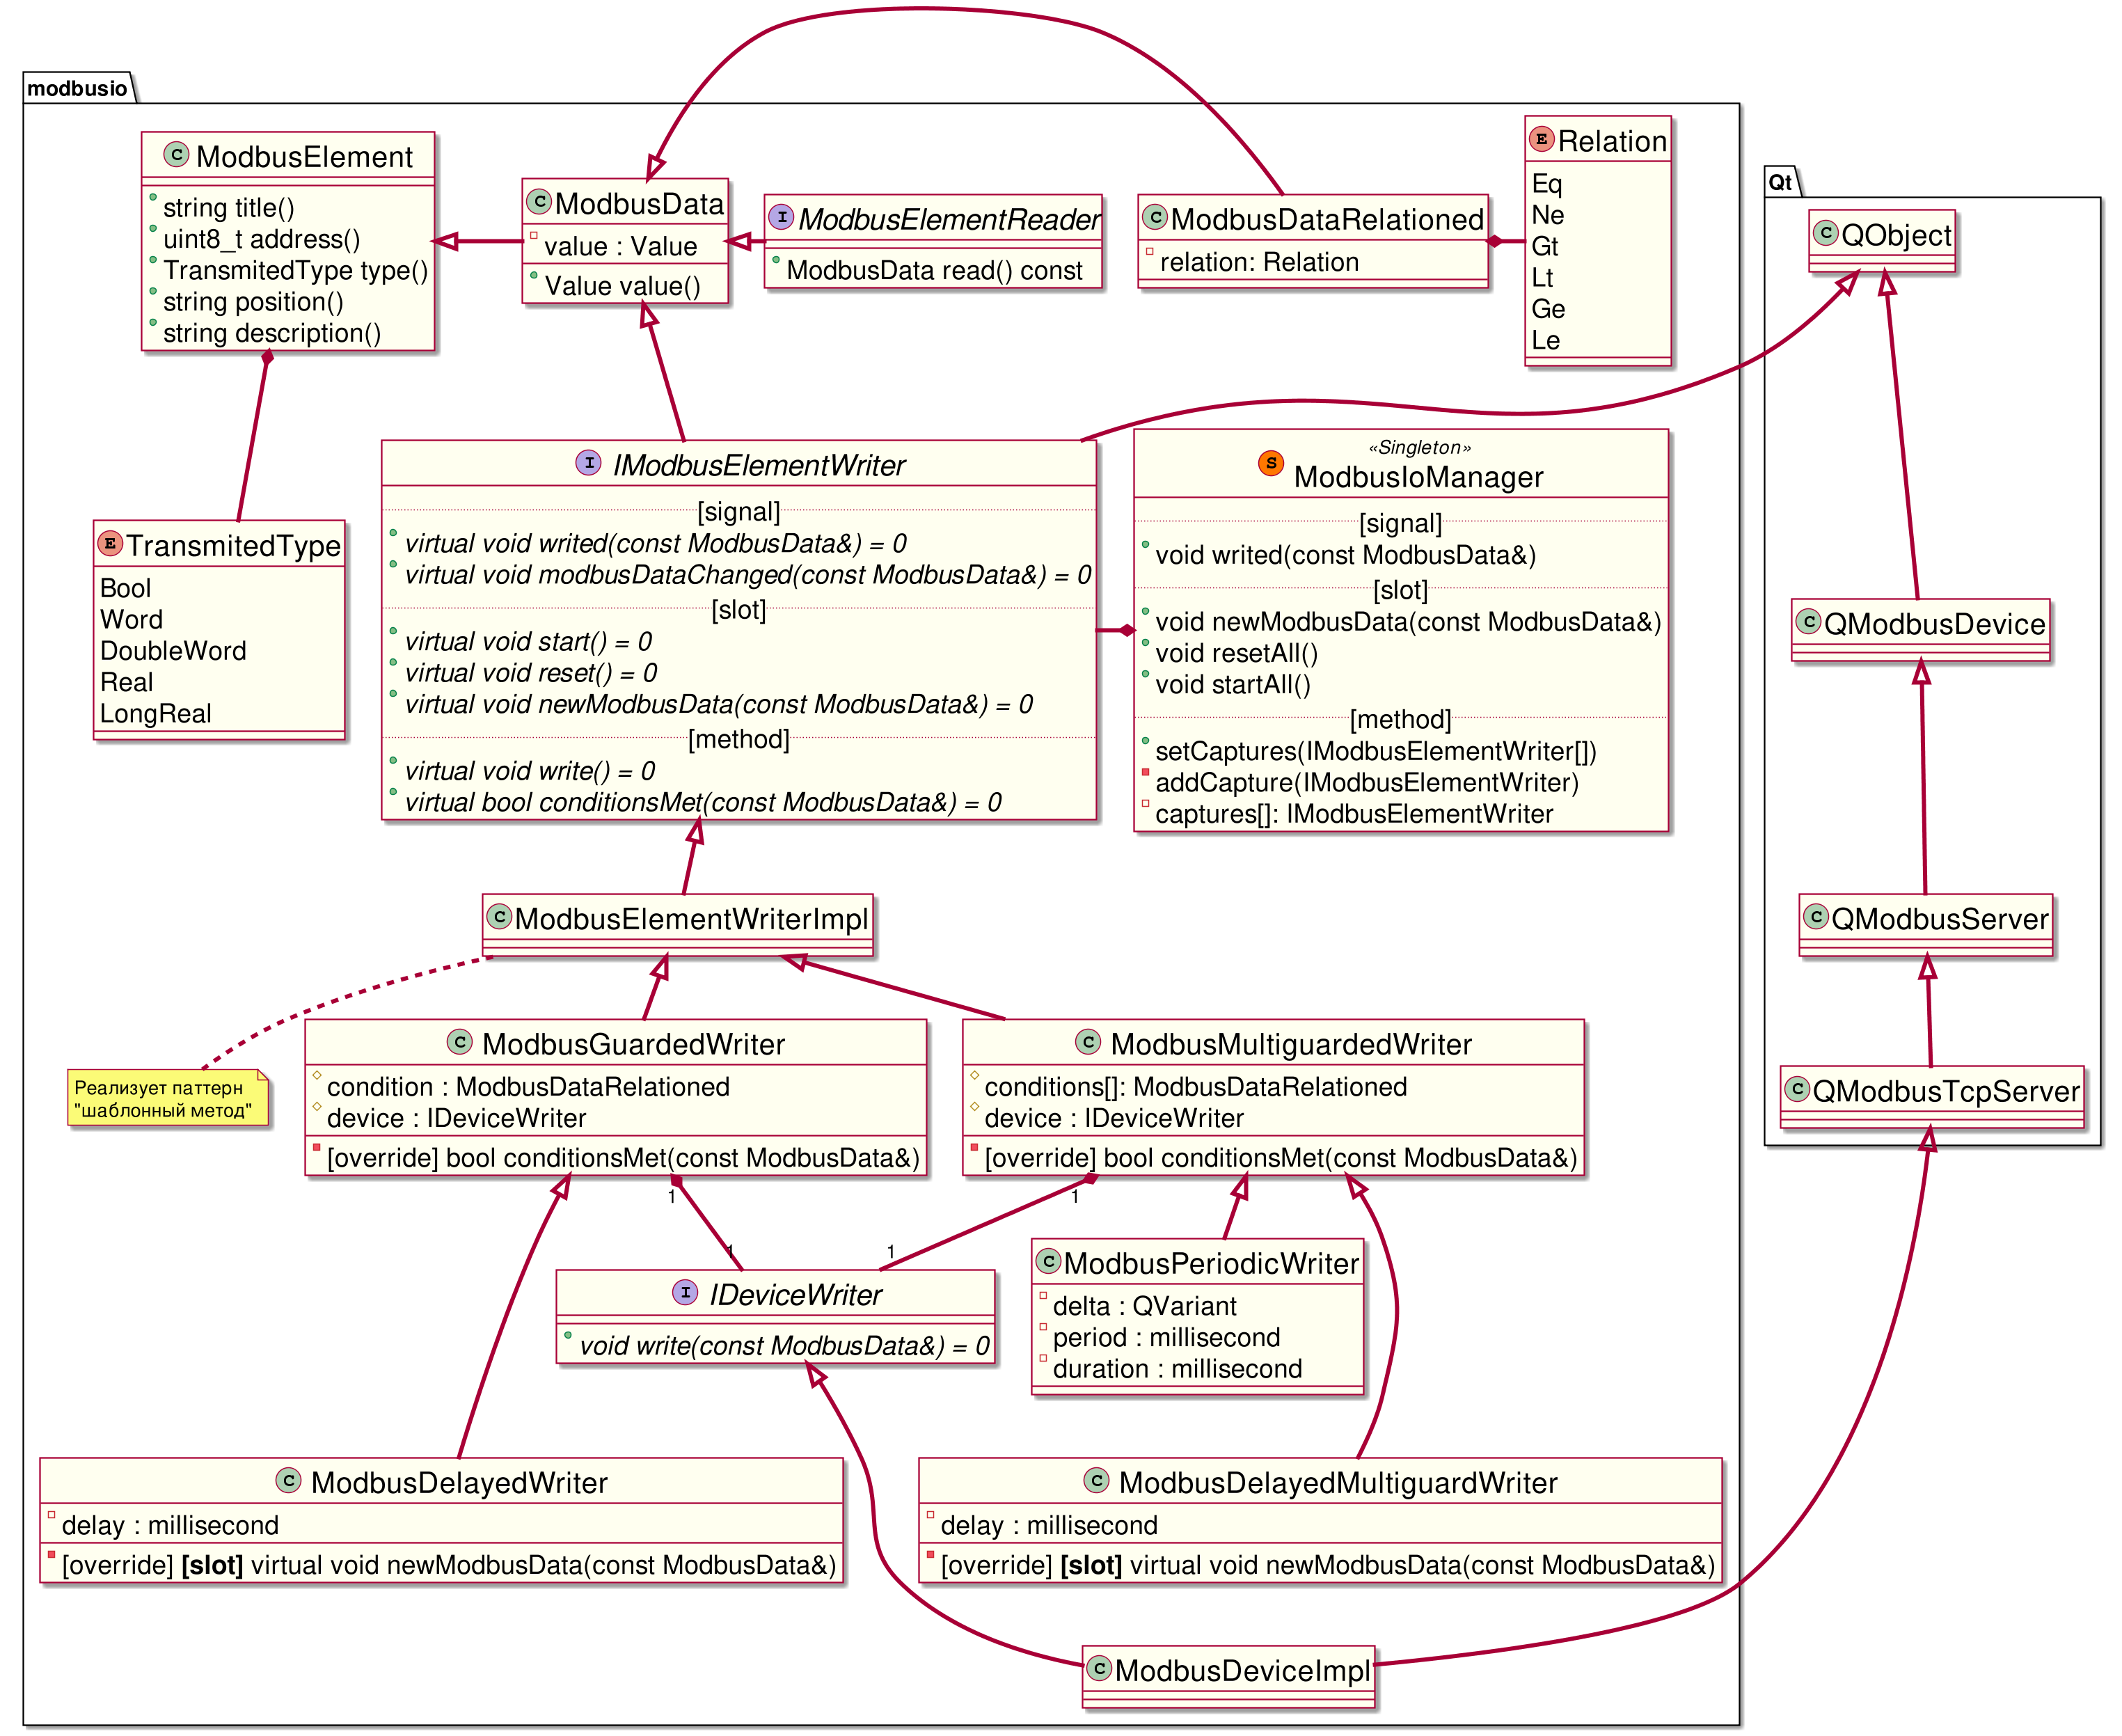
\includegraphics[height=.88\textheight,keepaspectratio]{modbus_class_relationship.png}
            \caption{\todo{UML диаграмма классов для имитатора передачи по сети Modbus}}\label{fig:modbus_class_uml}
        \end{figure}
    \end{center}
\end{landscape}
Базовый класс \texttt{ModbusElement} инкапсулирует в себе представление тега из раздела \ref{sec:modbus_tag}.
Для передачи данных между компонентами системы используется класс \texttt{ModbusData}, производный от \texttt{ModbusElement},
в котором появляется дополнительный член класса \texttt{value} для хранения значения.
Интерфейс \texttt{IModbusElementReader} введен для общности, но в данной работе представляет мало интереса, далее мы сосредоточимся 
на реализациях интерфейса \texttt{IModbusElementWriter}.



\subsection{Жизненный цикл компонента \texttt{IModbusElementWriter}}
Каждый экземпляр класса, реализующего интерфейс \texttt{IModbusElementWriter},
функционирует следующим образом, как показано на рисунке \ref{fig:imodbuselementwriter_activity} \cite[стр. 217]{book:oop:oop_analize}.
После создания, компонент находится в пассивном режиме ожидания, до тех пор пока не будет вызван
метод \texttt{IModbusElementWriter::start()}, после чего компонент подписывается на события шины данных по протоколу Modbus
и слушает сообщения об изменениях значений через слот \texttt{IModbusElementWriter::newModbusData()}.
При поступлении данных, удовлетворяющих условиям функции \texttt{IModbusElementWriter::conditionsMet()},
происходит запись значения через интерфейс \texttt{IDeviceWriter} (рисунок \ref{fig:modbus_device_imp}),
испускается сигнал \texttt{IModbusElementWriter::writed()},
а флаг \texttt{running} выставляется в значение \texttt{false}.
Таким образом, компонент отписывается от событий по шине данных.
Компонент может быть повторно подписан на события, через вызов метода \texttt{IModbusElementWriter::start()}.

\begin{center}
    \begin{figure}
        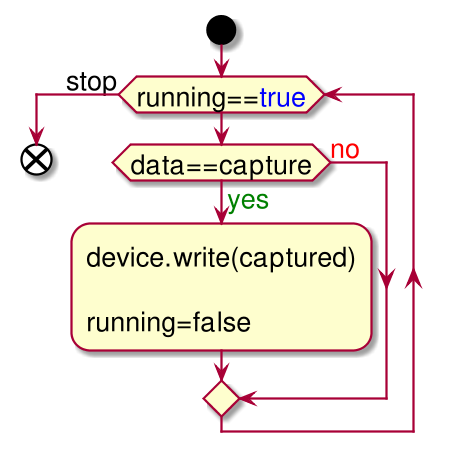
\includegraphics[width=.5\textwidth,keepaspectratio]{imodbuselementwriter_activity}
        \caption{Жизненный цикл компонента (см. также листинг \ref{lst:tmpl_method_writerimpl})}\label{fig:imodbuselementwriter_activity}
    \end{figure}
\end{center}


Класс \texttt{IModbusElementWriterImpl} (не показан на рисунке \ref{fig:modbus_class_uml})
реализует паттерн "Шаблонный метод" (Template method) \cite[стр. 309]{book:pattern:band_of_4},
определяя метод слота \texttt{IModbusElementWriter::newModbusData()}
и защищенный метод \texttt{IModbusElementWriter::write()} --- инвариантную последовательность операций,
определенную виртуальными методами, которые можно переопределить с помощью наследования \cite[стр. 170]{book:tdd:KentBeck}.

\lstinputlisting[
    language=C++,
    caption=Реализация контракта компонента (см. рисунок \ref{fig:imodbuselementwriter_activity}),
    label=lst:tmpl_method_writerimpl
        ]{Dissertation/listings/cpp/writerimpl_template_method.hpp}


\subsection{\todo{Условия перехода}}
Как видно из рисунка \ref{fig:modbus_class_uml} проверка условий записи описываются с помощью компонента типа
\texttt{ModbusDataRelationed} -- наследника класса \texttt{ModbusData}.
Этот класс содержит в себе \texttt{value} от родительского класса и правило отношения \texttt{Relation}.
При поступлении новых данных по шине Modbus происходит сравнение значений (листинг \ref{lst:comparator:compare}).
\lstinputlisting[
    language=C++,
    label=lst:comparator:compare,
    caption=Вспомогательный метод, использующийся при анализе поступающих данных.
        ]{Dissertation/listings/cpp/comparator.hpp}


Перейдем к более подробному рассмотрению реализаций интерфейса \texttt{IModbusElementWriter}.

\subsubsection{Запись с единичным условием}\label{sec:guard}
Циклограмма функционирования класса \texttt{ModbusGuardedWriter} приведена на рисунке \ref{fig:modbus_guarded_writed}.
Этот класс переопределяет метод родительского класса \texttt{IModbusElementWriter::conditionsMet()}.
\begin{center}
    \begin{figure}[h!]
        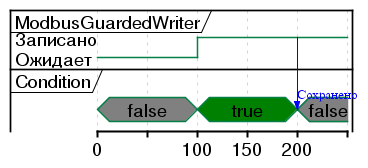
\includegraphics[width=.8\textwidth,keepaspectratio]{modbus_guarded_writer.png}
        \caption{Циклограмма записи значения при выполнении условия в момент времени $\tau_1=100$.}\label{fig:modbus_guarded_writed}
    \end{figure}
\end{center}
Как видно из рисунка выполнение условия происходит в момент времени $\tau_1=100$ условных единиц времени,
сразу же по переднему фронту происходит запись нового значения, которое сохраняется даже после окончания
выполнения логического условия \texttt{cond} в $\tau_2=300$.


\subsubsection{Запись со множественными условиями}
Циклограмма функционирования класса \texttt{ModbusMultiguardedWriter} приведена на рисунке \ref{fig:modbus_multiguarded_writed}.
Этот класс переопределяет метод родительского класса \texttt{IModbusElementWriterImpl::newModbusData()},
так как необходимо следить за множеством тегов через этот слот,
заполняется ассоциативный массив (например, \texttt{std::map<std::string, bool>} у которого ключем является
название тега \texttt{modbusio::ModbusElement::title()}, а значением результат \todo{надо посмотреть в коде \ldots})
\begin{center}
    \begin{figure}[h!]
        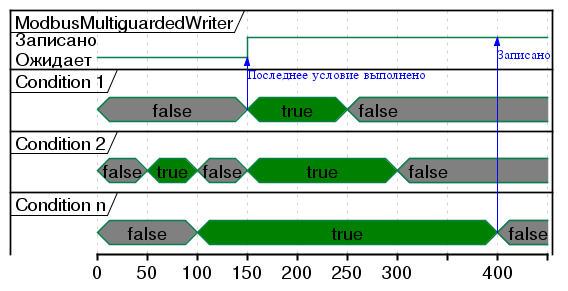
\includegraphics[width=.8\textwidth,keepaspectratio]{modbus_multiguarded_writer.png}
        \caption{Циклограмма записи значения при выполнении множественных условий.}\label{fig:modbus_multiguarded_writed}
    \end{figure}
\end{center}
Как видно из этого рисунка, значение не будет записано до тех пор, пока не будут
выполнены все условия, даже если после установления одного из условий оно меняется
(как показано для второго условия на 100 единице времени). Аналогично с \texttt{ModbusGuardedWriter}
после того как значение было записано, выполнение условий не контролируется, 
при этом записанное значение сохраняется, но может быть независимо изменено по другим причинам,
так как компонент больше не владеет ресурсом и отписывается от событий.


\subsubsection{Отложенная запись с единичным условием}
Циклограмма функционирования класса \texttt{ModbusDelayedWriter} приведена на рисунке \ref{fig:modbus_delayed_writer}.
Этот класс переопределяет метод родительского класса \texttt{ModbusGuardedWriter::conditionsMet()},
при выполнении условия которого запускается таймер на время \texttt{\_delay},
по окончании которого происходит запись значения.
\begin{lstlisting}[language=C++]
    ModbusDelayedWriter::conditionsMet(const modbus::ModbusData& data)
        if (_running && !_timerRun) {
            _timerRun = true;
            QTimer::singleShot(_delay, this, &IModbusElementWriter::write);
        }
\end{lstlisting}

\begin{center}
    \begin{figure}[h!]
        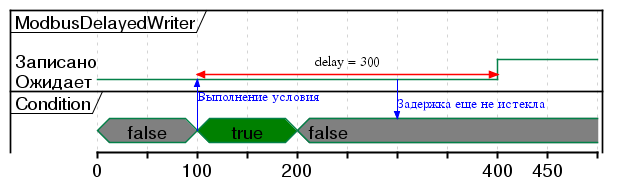
\includegraphics[width=.8\textwidth,keepaspectratio]{modbus_delayed_writer.png}
        \caption{Циклограмма отложенной записи значения при выполнении единственного условия.}\label{fig:modbus_delayed_writer}
    \end{figure}
\end{center}
Класс позволяет устанавливать значение после выполнения условия и по истечению задержки $\tau$.
По окончании таймера на запись значение выражения \texttt{Condition} не анализируется
и запись происходит в любом случае.


\subsubsection{Отложенная запись со множеством условий}
Циклограмма функционирования класса \texttt{ModbusDelayedMultiguardWriter} приведена на рисунке \ref{fig:modbus_delayed_multiguarded_writer}.
\todo{Надо посмотреть код, чтобы точно сказать какой метод переопределен \ldots}
\begin{center}
    \begin{figure}[h!]
        \includegraphics[width=.8\textwidth,keepaspectratio]%
            {modbus_delayed_multiguarded_writer.png}
        \caption{Циклограмма отложенной записи значения при выполнении множественных условий.}\label{fig:modbus_delayed_multiguarded_writer}
    \end{figure}
\end{center}


\subsubsection{Периодическая запись}
Данный компонент предназначен для реализации периодических событий, как показано на диаграмме \ref{fig:modbus_periodic_writer}.
При захвате управления дискретной переменной, ее значение инвертируется каждый период
$f_i(x; \tau) = \lnot f_{i-1}(x; \tau), f(x; \tau) \in \{True, False\}$
(на графике сверху захвачен булевский тег, период равен 25 единиц времени).
При захвате вещественной переменной значение меняется по закону
$f_i(x,\Delta x; \tau) = f_{i-1}(x,\Delta x; \tau) + \Delta x, \Delta x \in \mathcal{R}$
(на графике снизу период равен 50 единиц времени, $\Delta x = 10$ на 200 единиц времени).
\begin{center}
    \begin{figure}[h!]
        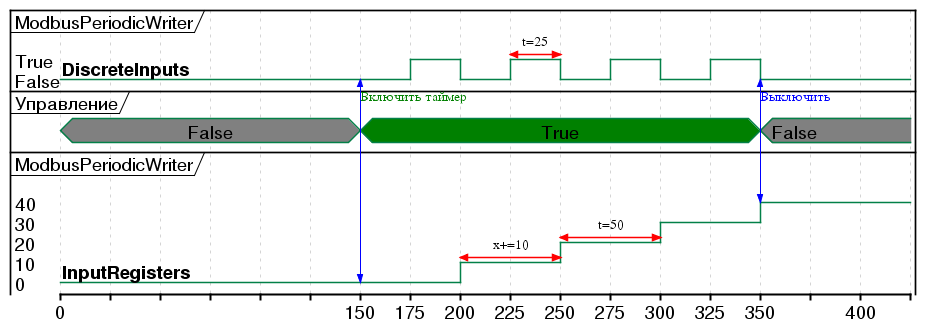
\includegraphics[width=.8\textwidth,keepaspectratio]{modbus_periodic_writer.png}
        \caption{Циклограмма периодической записи значения.}\label{fig:modbus_periodic_writer}
    \end{figure}
\end{center}
Этот компонент используется, например, для управления значениями количества оборотов,
количества транзакций и пакетов, переданных от контроллера к программе верхнего уровня,
при захвате вещественных переменной.
Очевидно, что приращение $\Delta x$ может быть как положительным, так и отрицательным.

Если в конфигурации сценария (листинг \ref{lst:modbus_periodic_writer_xml}) имеется аттрибут
\texttt{duration}, компонент будет работать от выполнения условий до окончания указанной длительности.
В противном случае обновление значений будет происходить до момента прекращения работы
\texttt{ModbusIoManager::resetAll()}.


\subsection{Реализация интерфейса \texttt{IDeviceWriter}}
При реализации интерфейса \texttt{IDeviceWriter} используется возможность множественного наследование языка программирования \cpp,
одним из родителей является интерфейс \texttt{IDeviceWriter},
а вторым --- класс библиотеки \texttt{Qt}, обеспечивающий реализацию физической передачи информации по протоколу Modbus
\texttt{QModbusTcpServer}, так как обмен происходит по разновидности протокола Modbus TCP/IP.
Упрощенная реализация показана в листинге \ref{lst:imodbus_device_impl}.
\begin{center}
    \begin{figure}
        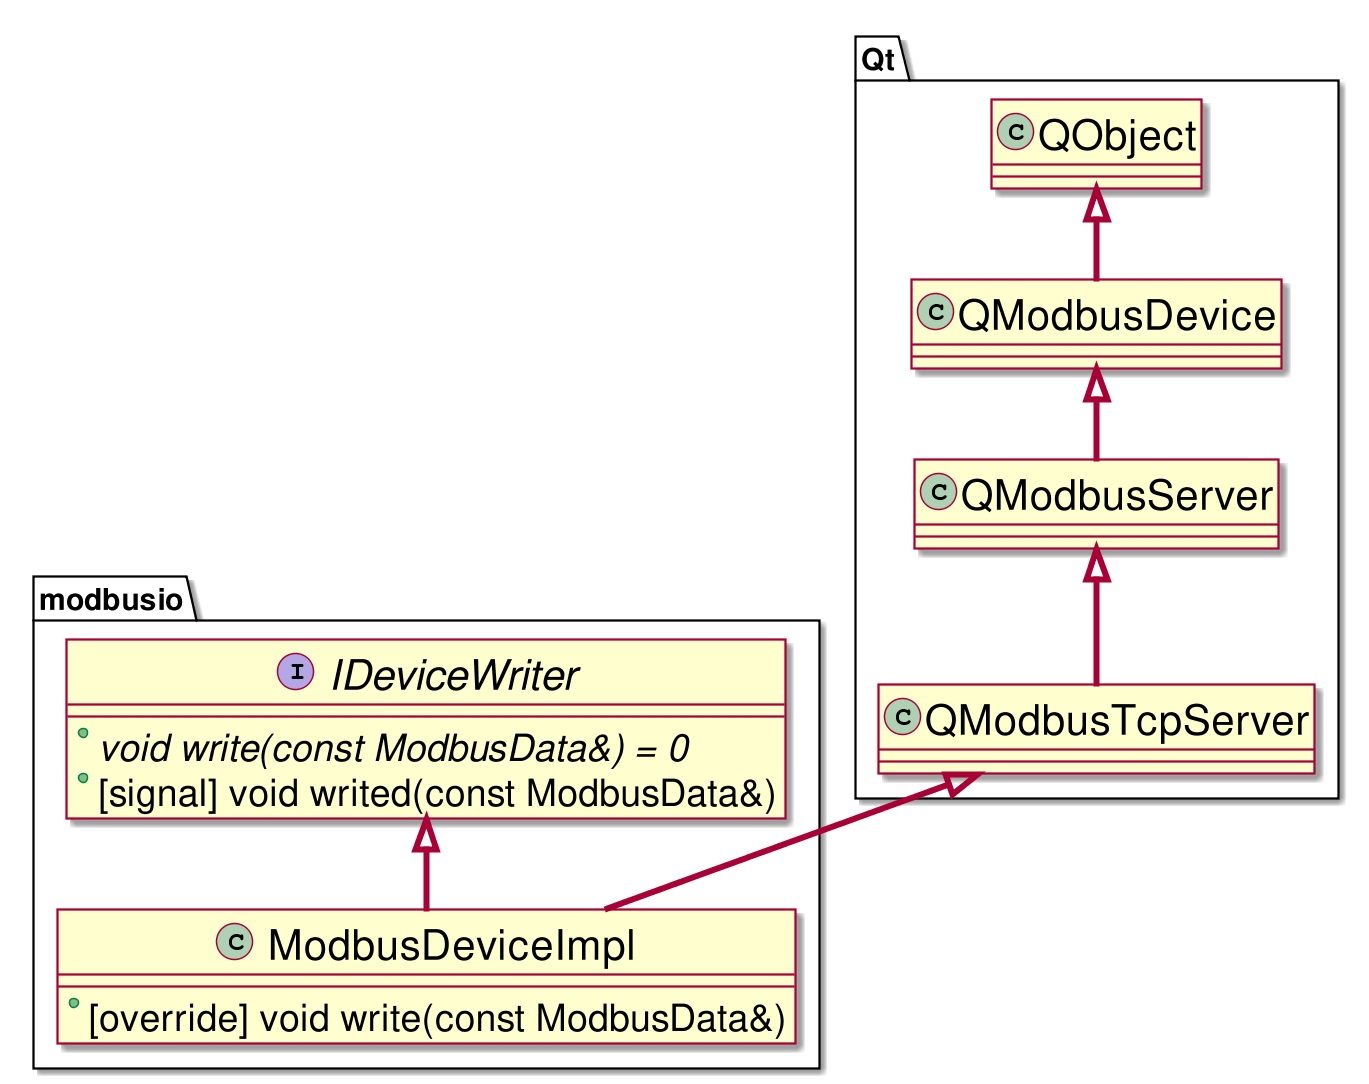
\includegraphics[width=.9\textwidth,keepaspectratio]{modbus_device_impl.png}
        \caption{Реализация устройства для записи значений по протоколу Modbus}\label{fig:modbus_device_imp}
    \end{figure}
\end{center}
\lstinputlisting[
    language=C++,
    caption=Простейшая реализация \texttt{IDeviceWriter} устройства,
    label=lst:imodbus_device_impl]
        {Dissertation/listings/cpp/dummydeviceimpl.hpp}
Таким образом используется интерфейс вместо конкретной реализации \cite[стр. 47-48]{book:pattern:head_first}


\subsection{Описание конфигурационного файла для компонентов интерфейса \texttt{IModbusElementWriter}}
Каждая группа должна быть помещена в корневой элемент \texttt{Scenario},
как показано в листинге \ref{lst:modbus_scenario_example_diagram} приложения \ref{app:sec:modbus_scenario_example_diagram}.

Каждый компонент помещается внутри тега \texttt{Writer},
с обязательным текстовым аттрибутом \texttt{tag}, который указывает каким ресурсом владеет данный компонент
и обязательным аттрибутом \texttt{value}, который выполняет различную роль в зависимости от назначения компонента (см. листинг \ref{lst:modbus_tags_scenario_configs}).
Одновременно владеть одним и тем же ресурсом могут несколько компонентов (как будет показано ниже).
Далее следует секция условий, которая присутствует даже для компонентов \texttt{ModbusGuardedWriter} и \texttt{ModbusDelayedWriter},
для общности парсера конфигурационного файла.
Каждое условие описывается логической операцией отношения \texttt{relation} для смежного параметра, указанного в обязательном поле \texttt{tag} и
связанного с ним значения \texttt{value}.
Элемент \texttt{relation} принимает одно из следующих значений:
\texttt{eq} ($=$),
\texttt{ne} ($\neq$),
\texttt{gt} ($>$),
\texttt{lt} ($<$),
\texttt{ge} ($\geq$),
\texttt{le} ($\leq$), по аналогии с обозначениями в языке Fortran.
Для дискретных (булевых) переменных необязательно указывать отношения типа \texttt{eq},
если интересует отношение равенства, отношение \texttt{ne} неравенства же необходимо указывать явным образом.
Необязательным полем является поле \texttt{Description}, в котором размещается информация для
обозначения назначения компонента в сценарии, а так же могут располагаться другие произвольные текстовые данные.

\subsubsection{ModbusGuardedWriter}
Рассмотрим более подробно описание компонента для компонента с единичным условием записи,
который размещается в элементе \texttt{Guarded}:
\lstinputlisting[
    language=MyXML,
    caption=Пример конфигурации \texttt{ModbusGuardedWriter},
    label=lst:modbus_guarded_writer_xml]
        {Dissertation/listings/xml/guarded.xml}
Захватывается управление над тегом \texttt{A1}, которой будет присвоено значение 160
при выполнении условия \texttt{R1 = true}.


\subsubsection{ModbusMultiguardedWriter}
Для описания компонента со множественными условиями, используется следующий формат,
который размещается в элементе \texttt{Multiguarded}:
\lstinputlisting[
    language=MyXML,
    caption=Пример конфигурации \texttt{ModbusMultiguardedWriter},
    label=lst:modbus_multiguarded_writer_xml]
        {Dissertation/listings/xml/multiguarded.xml}
Переменной \texttt{Regime} будет присвоено значение 1, как только 
одновременно будет выполнено два условия: $Regime = 1: \{A1 \ge 150 \wedge C1 = true\}$.

\subsubsection{ModbusDelayedWriter и ModbusDelayedMultiguardWriter}
Компоненты этого типа располагаются в окружении тегов элементов \texttt{Delayed} и \texttt{Multidelayed}, соответственно.
\lstinputlisting[
    language=MyXML,
    caption=Пример конфигурации \texttt{ModbusDelayedWriter} и \texttt{ModbusDelayedMultiguardWriter},
    label=lst:modbus_delayed_writer_xml]
        {Dissertation/listings/xml/delayed.xml}
Захватывается управление переменной \texttt{PP\_1}, которой будет установлено значение \texttt{true}
через 50 единиц времени, как только будут выполнены два условия:
$PP\_1 = \mbox{true}: \{R1 = true \wedge A1 \le 150\}$.


\subsubsection{ModbusPeriodicWriter}
Данный компонент располагается внутри элемента \texttt{Period} в конфигурационном файле сценария.
\lstinputlisting[
    language=MyXML,
    caption=Пример конфигурации \texttt{ModbusPeriodicWriter},
    label=lst:modbus_periodic_writer_xml]
        {Dissertation/listings/xml/periodic.xml}
В данном примере дистанция, ассоциированная с переменной \texttt{Distance}, увеличивается на 100 единиц каждые 1000 единиц времени,
при выполнении ряда условий, а именно: $\{C1 = true \wedge A1 > 100 \wedge A1 \le 150 \}$ или
увеличивается на теже 100 единиц, но с периодом 500 единиц, когда достигаются следующие условия:
$\{C1 = true \wedge A1 > 150\}$
Отметим, что для этого компонента начальное значение устанавливается с помощью аттрибута \texttt{value}
при вызове метода \texttt{IModbusElementWriter::start()}.


\subsection{Сводная таблица наследников \texttt{IModbusElementWriter}}
\begin{table}[]
\caption{\todo{Сводная таблица наследников}}\label{tbl:IModbusElementWriterImpl}
\begin{tabular}{|l|c|c|c|c|c|c|c|c|}
\hline
    \multicolumn{1}{|c|}{\multirow{2}{*}{Наследники}} &
    \multicolumn{6}{c|}{\textbf{Аттрибуты}} &
    \multicolumn{2}{c|}{\textbf{Переопределенные методы наследника}} \\ \cline{2-8} 
    \multicolumn{1}{|c|}{}     &
        \rotatebox{90}{tag} & \rotatebox{90}{value}  & \rotatebox{90}{delay}  & \rotatebox{90}{period} &
        \rotatebox{90}{delta} & \rotatebox{90}{duration} &
        \rotatebox{90}{conditionsMet} & \rotatebox{90}{newModbusData} \\ \hline
    \texttt{ModbusGuardedWriter}              & +    & +      & -      & -      & - &-     & + & -  \\ \hline
    \texttt{ModbusMultiguardedWriter}         & +    & +      & -      & -      & - &-     & + & -  \\ \hline
    \texttt{ModbusDelayedWriter}              & +    & +      & +      & -      & - &-     & - & +  \\ \hline
    \texttt{ModbusDelayedMultiguardWriter}    & +    & +      & +      & -      & - &-     & - & +  \\ \hline
    \texttt{ModbusPeriodicWriter}             & +    & +      & -      & +      & + &$\pm$ & + & -  \\ \hline
\end{tabular}
\end{table}


\subsection{Менеджер состояний}
Для управления компонентами имитатора используется менеджер \texttt{ModbusIoManager}. Установка компонентов производится с помощью экземпляра класса \texttt{ScenarioParser}, реализующего интерфейс \texttt{IParser}.
Этот интерфейс является общим для как для чтения файла сценария (\ref{lst:modbus_scenario_example_diagram}),
так и для файла тегов (листинг \ref{lst::modbus_tags_example}).
После чтения конфигурации, ее необходимо проверить, что каждый тег $t_i$
компонента, управление над которым захватывает и условия выполнения переходов, является элементов множества \texttt{ModbusTags},
то есть $\forall t_i \in \mbox{ModbusTags}$.
\begin{center}
    \begin{figure}
        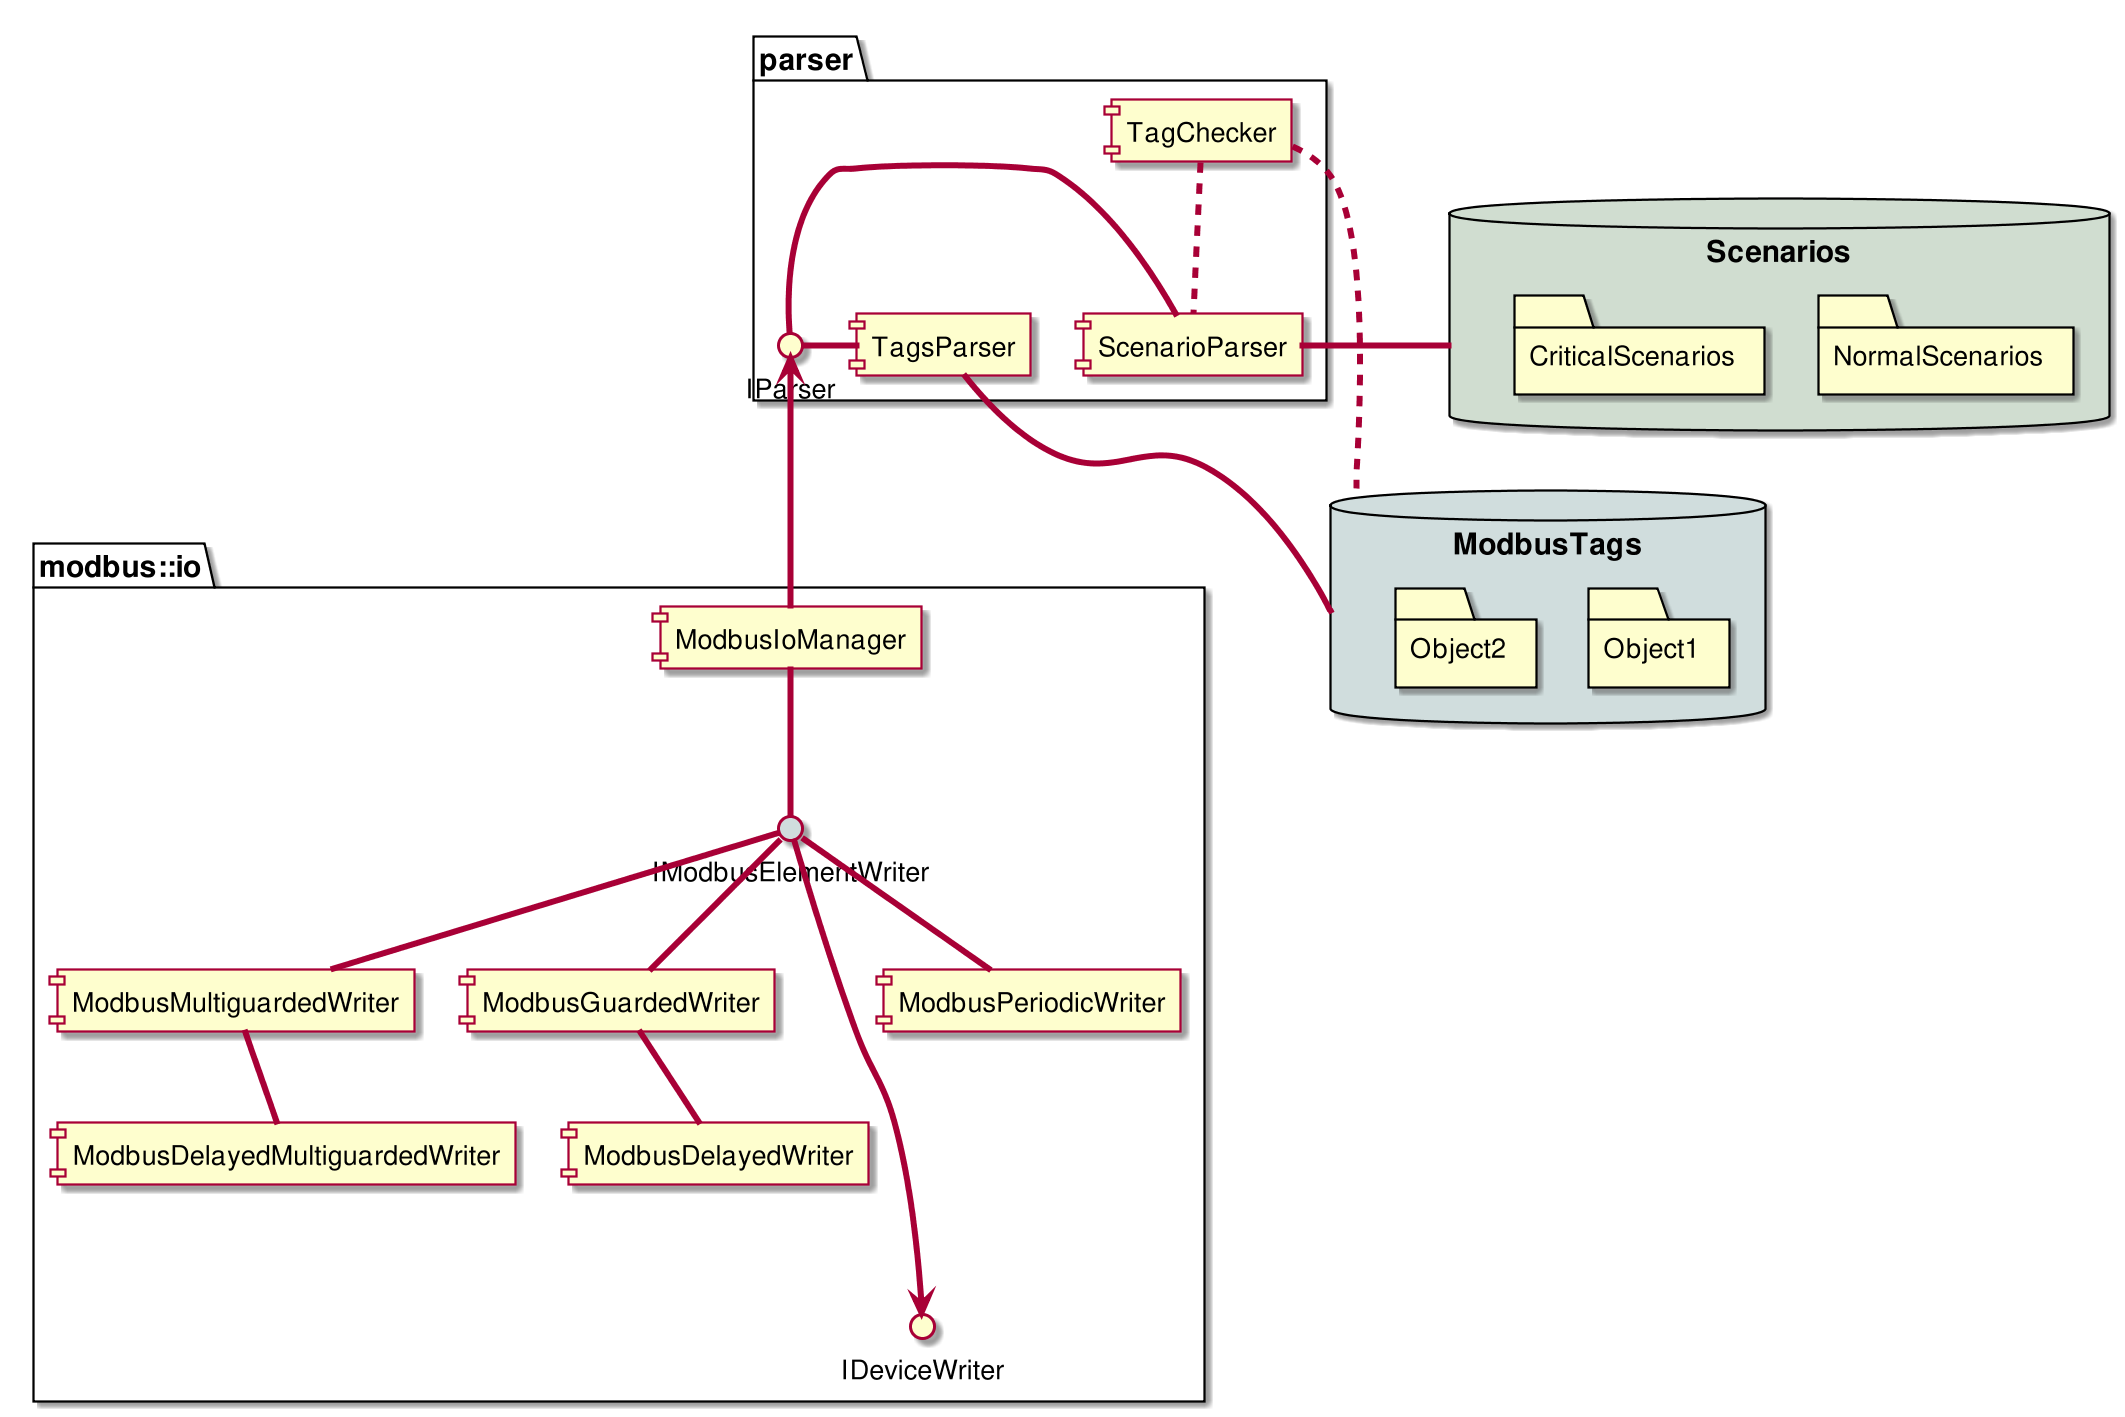
\includegraphics[width=.9\textwidth,keepaspectratio]{modbus_class_components}
        \caption{Композиция классов менеджера сценариев}\label{fig:modbus_class_components}
    \end{figure}
\end{center}

\begin{center}
    \begin{figure}
        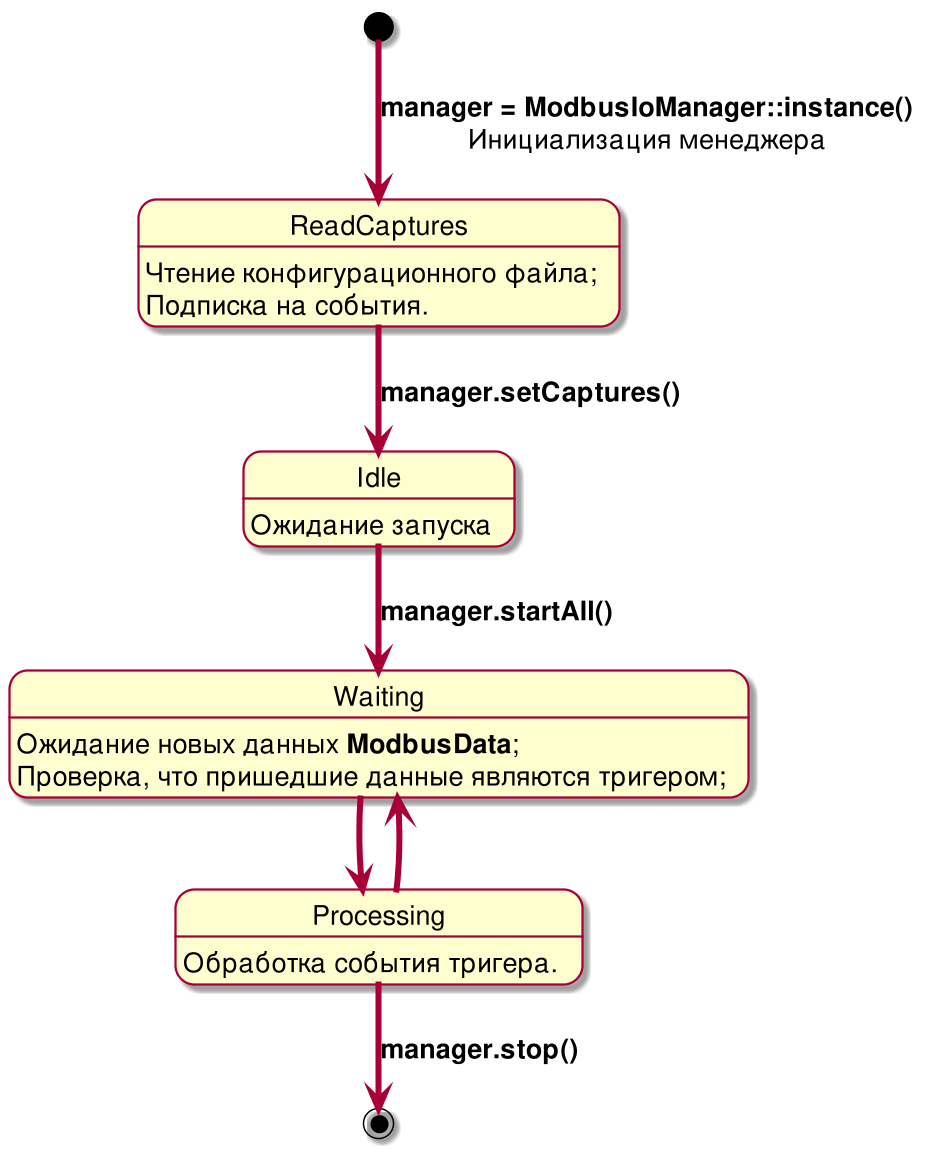
\includegraphics[width=.9\textwidth,keepaspectratio]{modbusiomanager_state_diagram}
        \caption{\todo{Жизненный цикл ModbusIoManager}}\label{fig:modbusiomanager_state_diagram}
    \end{figure}
\end{center}

Последовательность действий показана на рисунке \ref{fig:top_level_sequence} \cite[стр. 239]{book:oop:oop_analize}
\begin{center}
    \begin{figure}
        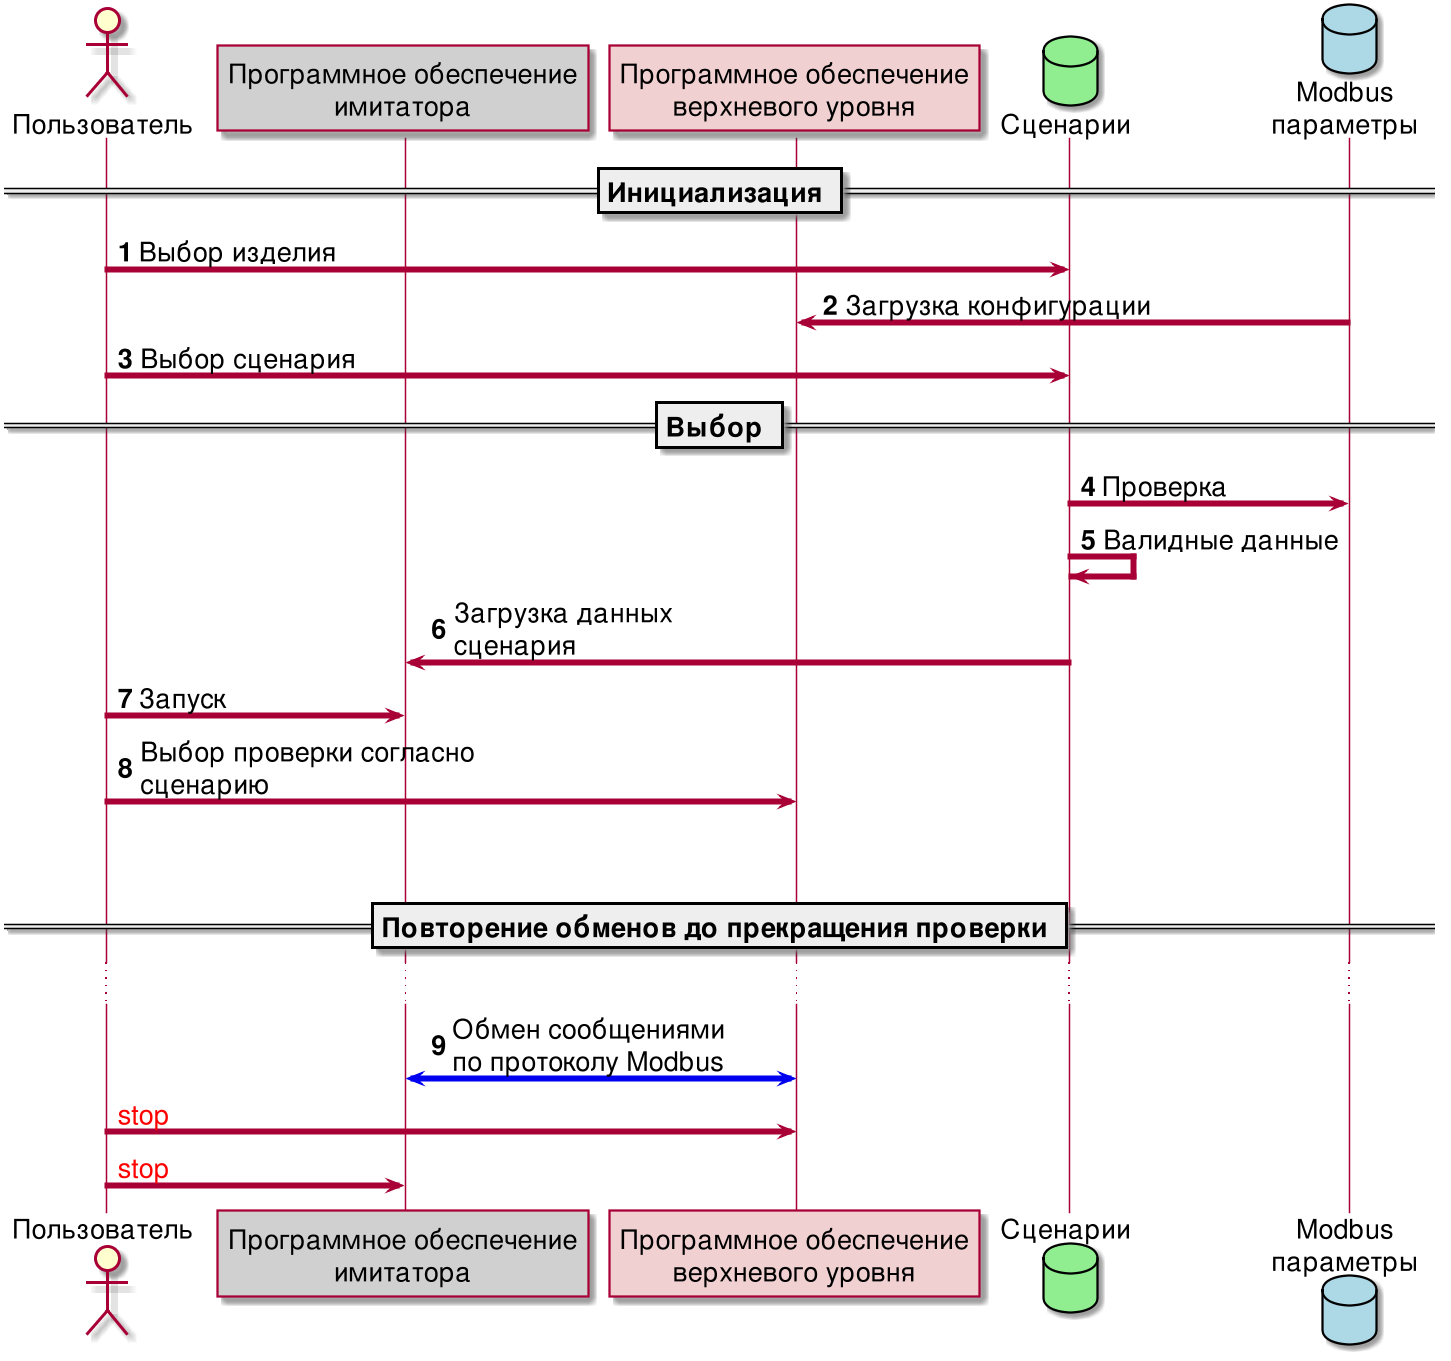
\includegraphics[width=.9\textwidth,keepaspectratio]{top_level.png}
        \caption{Последовательность действий при работе с имитатором}\label{fig:top_level_sequence}
    \end{figure}
\end{center}

\clearpage
\section{Пример композиции для простейшего сценария}

Рассмотрим пример сценария на основе множества Modbus тегов из листинга \ref{lst:modbus_tags_example},
циклограмма которого представлена на рисунке \ref{fig:modbus_scenario_example_diagram},
сценарий приведен в листинге \ref{lst:modbus_scenario_example_diagram} в разделе приложения \ref{app:sec:modbus_scenario_example_diagram}.
% Схема разметки приведена в листинге \ref{lst:modbus_tags_scenario_configs}.

\begin{landscape}
    \begin{center}
        \begin{figure}
            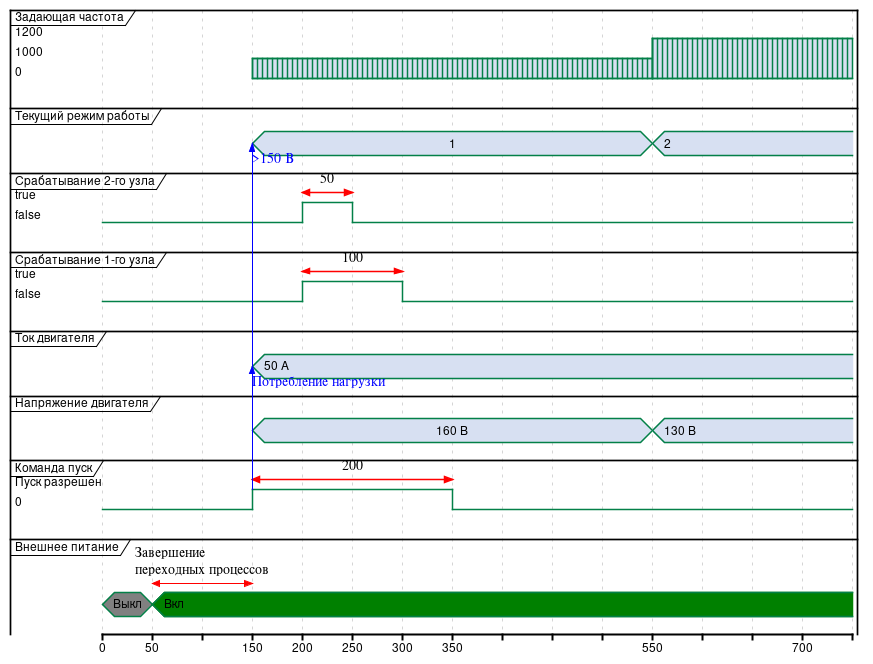
\includegraphics[height=.8\textheight,keepaspectratio]{modbus_scenario_example_diagram.png}
            \caption{Пример использования классов.}\label{fig:modbus_scenario_example_diagram}
        \end{figure}
    \end{center}
\end{landscape}


\section*{Выводы}
Таким образом можно использовать унифицированный способ представления сценария для имитатора \ldots



% \section{Распределение ролей}
% На стороне СК создается экземпляр клиента сети modbus,
% имитатор представляет сервер (см. главу \ref{ch:ch2}).
% \section{Конфигурационный файл}\label{sec:ch2/sec1}
% Общее пространство данных modbus у ПО СК и имитатора \ldots
% \section{Паттерн MVC}
% Поверх множества данных modbus используется паттерн проектирования модель-вид-контроллер \cite{book:pattern:band_of_4}.
% Библиотека Qt позволяет создавать модель данных, наследуя поведение от \lstinline[language=C]!QAbstractTableModel!,
% переобпределяя реализацию методов для чтения-записи данных в модель.
% \subsection{Пояснение в реализации методов}
% \subsection{Преимущества такого подхода}
